\section{Theorie}

Mithilfe von Brückenschaltungen lassen sich Größen, die durch einen elektrischen/komplexen Widerstand ausgedrückt werden können, eindeutig messen. 
\begin{figure}[h]
  \centering
  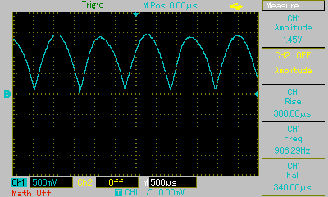
\includegraphics[height=4cm]{Grafiken/1.pdf}
  \caption{einfache Brückenschaltung. \cite{1}}
  \label{fig:Brücke}
\end{figure}
In einer Brückenschaltung herrscht eine Potentialdifferenz zwischen zwei Punkten. Der Strom teilt sich dabei wie in \ref{fig:Brücke} in zwei Äste auf. 
Zwischen A und B wird die Brückenspannung gemessen. Um diese zu berechnen, werden die Kirchhoffschen Gesetze verwendet:
\\
1. die Summe aller eingehenden und ausgehenden Ströme an einem Knoten ist gleich Null
\begin{equation}
	\sum_k I_\text{k} = 0
\end{equation}
\\
2. die Summe aller Spannungen eines geschlossenen Stromkreises ist unter Beachtung des Vorzeichens Null
\begin{equation}
	\sum_k U_\text{k} = 0
\end{equation}
\\
So ergibt sich dann für die Brückenspannung $U_\text{Br}$:
\begin{equation}
	U_\text{Br} = \frac{R_2R_3 - R_1R_4}{(R_3+R_4)(R_1+R_2)}U_\text{S}
\end{equation}
Verschwindet die Brückenspannung, so erhält man die Formel eine abgeglichenen Brücke:
\begin{equation}
	R_1R_4 = R_2R_3
\end{equation}
Je genauer die bekannten Widerstände sind, desto genauer wird auch die Messung des unbekannten Widerstandes.
Verwendet man, aufgrund von Kapazitäten und Induktivitäten komplexe Widerstände, so muss für diesen Fall die Brückenspannung nach Betrag und Phase Null werden. 

\subsection{Wheatstonesche Brücke}

\begin{figure}[h]
  \centering
  \includegraphics[height=4cm]{Grafiken/Wheatstone.pdf}
  \caption{Wheatstonesche Brückenschaltung. \cite{1}}
  \label{fig:Wheatstone}
\end{figure}
In der Schaltung \ref{fig:Wheatstone} befinden sich nur ohmsche Widerstände. Mithilfe dieser Schaltung kann der Widerstand $R_\text{x}$ bestimmt werden:
\begin{equation}
	R_\text{x} = R_2\frac{R_3}{R_4}
\end{equation}
Somit wird nur das Verhältnis von $R_3$ und $R_4$ benötigt, weshalb diese in einem Potentiometer vereint sind.
Diese Schaltung kann sowohl mit Gleich- als auch mit Wechselstrom betrieben werden.

\subsection{Kapazitätsmessbrücke}

\begin{figure}[h]
  \centering
  \includegraphics[height=4cm]{Grafiken/Kapazität.pdf}
  \caption{Schaltung einer Kapazitätsmessbrücke. \cite{1}}
  \label{fig:Kapazität}
\end{figure}
Reale Kondensatoren bestehen aus einer Kapazität und einem Widerstand, der einen Teil der durch sie hindurchfließenden Energie in Wärme umwandelt, abgebildet in \ref{fig:Kapazität} durch $C_x$ und $R_\text{x}$. Um $C_\text{x}$ zu bestimmen, muss daher noch ein Widerstand $R_2$ und eine Kapazität $C_2$ hinzugeschaltet werden. 
Somit gilt: 
\begin{gather}
	C_\text{x} = C_2\frac{R_4}{R_3} \\
	R_\text{x} = R_2\frac{R_3}{R_4}
\end{gather}

\subsection{Induktivitätsmessbrücke}

\begin{figure}[h]
  \centering
  \includegraphics[height=4cm]{Grafiken/Induktivität.pdf}
  \caption{Schaltung einer Induktivitätsmessbrücke. \cite{1}}
  \label{fig:Induktivität}
\end{figure}
Reale Spulen bestehen aus einer Induktivität und einem Widerstand, der einen Teil der in ihnen enthaltenden magnetischen Feldenergie in Wärme umwandelt, abgebildet in \ref{fig:Induktivität} durch $L_\text{x}$ und $R_\text{x}$. Wie bei der Kapazitätsmessbrücke werden zur Bestimmung von $L_\text{x}$ die Induktivität $L_2$ und der Widerstand $R_2$ hinzugeschaltet.
\begin{gather}
	L_\text{x} = L_2\frac{R_3}{R_4} \\
	R_\text{x} = R_2\frac{R_3}{R_4}
\end{gather}
Die Spule $L_2$ sollte so geringe Verluste wie möglich besitzen, damit eine genaue Messung gewährleistet werden kann. Dies ist in der Praxis, vor allem bei niedrigen Frequenzen, meist nicht möglich.

\subsection{Maxwell-Brücke}

\begin{figure}[h]
  \centering
  \includegraphics[height=4cm]{Grafiken/Maxwell.pdf}
  \caption{Schaltung einer Maxwell-Brücke. \cite{1}}
  \label{fig:Maxwell}
\end{figure}
Mithilfe der Maxwell-Brücke (siehe \ref{fig:Maxwell}) können ebenso Induktivitäten gemessen werden. Ihr Vorteil liegt jedoch darin, dass auf die Induktivität $L_2$ verzichtet werden kann und stattdessen die Kapazität $C_4$ verwendet wird. Diese Kapazität hat einen deutlich geringeren Wirkwiderstand, weshalb $L_\text{x}$ genauer gemessen werden kann. 
Somit folgt:
\begin{gather}
	L_\text{x} = R_2R_3C_4 \\
	R_\text{x} = R_2\frac{R_3}{R_4}
\end{gather}
\\
\\
In den vorherigen Abgleichungen wurde die Frequenz der Speisespannung nicht beachtet, weshalb angenommen wurde, dass die Brücken bei allen Frequenzen abgleichbar sind. In der Praxis ist dies jedoch nicht der Fall. Vielmehr gibt es nur einen bestimmten Frequenzbereich, in dem der Abgleich unter optimalen Bedingungen möglich ist. Wird die Kreisfrequenz $\omega$ zu hoch gewählt, so werden die Streukapazitäten zu groß, weshalb ein Abgleich nicht mehr möglich ist. Wird $\omega$ hingegen zu klein gewählt, so dauert es mehrere Periodendauern bis eine stationäre Brückenspannung auftritt. 
Eine optimale Frequenz wird erreicht, wenn Wirk- und Blindwiderstände die gleiche Größenordnung besitzen.

\subsection{Wien-Robinson-Brücke}

\begin{figure}[h]
  \centering
  \includegraphics[height=4cm]{Grafiken/Wien.pdf}
  \caption{Schaltung einer Wien-Robinson-Brücke. \cite{1}}
  \label{fig:Wien}
\end{figure}

Mithilfe der Wien-Robinson-Brücke (siehe \ref{fig:Wien}) sollen keine Widerstände gemessen werden. Sie dient als elektronischer Filter für ein kontinuierliches Frequenzspektrum. Sie entfernt die Schwingungen mit der Kreisfrequenz $\omega_0$.
Dies wird durch das Verhältnis von Brückenspannung und Speisespannung deutlich:
\begin{equation}
	\biggl | \frac{U_\text{Br, eff}}{U_\text{S}} \biggr |^2 = \frac{(\omega^2R^2C^2 - 1)^2}{9[(1-\omega^2R^2C^2)^2 + 9 \omega^2R^2C^2]}
\end{equation}

Für $\omega_0 = \frac{1}{RC}$ verschwindet die Brückenspannung.
Mit 
\begin{equation}
	\Omega = \frac{\omega}{\omega_0} \notag
\end{equation}
folgt:
\begin{equation}
	\biggl | \frac{U_\text{Br, eff}}{U_\text{S}} \biggr |^2 = \frac{1}{9}\frac{(\Omega^2 - 1)^2}{(1-\Omega^2)^2 + 9\Omega^2}
\end{equation}

Mithilfe der Wien-Robinson-Brücke kann der sogenannte Klirrfaktor bestimmt werden. Dieser Faktor beschreibt den Anteil der Oberwellen im Verhältnis zur Grundwelle einer angelegten Sinusspannung. In der Theorie sind diese Oberwellen nicht vorhanden, in der Praxis treten diese jedoch auf. Somit ist die Kleinheit des Klirrfaktors ein Maß für die Güte eines Sinusgenerators. 

\subsection{TT-Brücke}

\begin{figure}[h]
  \centering
  \includegraphics[height=4cm]{Grafiken/TT.pdf}
  \caption{Schaltung einer TT-Brücke. \cite{1}}
  \label{fig:TT}
\end{figure}
Die TT-Brücke hat denselben Zweck wie die Wien-Robinson-Brücke, hat jedoch den Vorteil, dass sowohl Eingangs-, als auch Ausgangsspannung gegen Masse angeschlossen werden kann (siehe Abbildung \ref{fig:TT}). 
Daraus ergibt sich dann:
\begin{equation}
	\biggl | \frac{U_\text{Br, eff}}{U_\text{S}} \biggr |^2 = \frac{(\Omega^2 -1)^2}{(1- \Omega^2)^2 + 16\Omega^2}
\end{equation}
Der Frequenzverlauf der TT-Brücke ähnelt stark dem der Wien-Robinson-Brücke.
